\documentclass[11pt, a4paper]{article}
\usepackage{pdfpages}
\usepackage{parallel}
\usepackage[T2A]{fontenc}
%\usepackage{ucs}
\usepackage[utf8]{inputenc}
\usepackage[english,russian]{babel}
\usepackage{hyperref}
\usepackage{rotating}
\usepackage[inner=2cm,top=1.8cm,outer=2cm,bottom=2.3cm,nohead]{geometry}
%\usepackage{listings}
\usepackage{graphicx}
\usepackage{wrapfig}
\usepackage{longtable}
\usepackage{indentfirst}
\usepackage{array}
\usepackage{tikzsymbols}
\usepackage{soul}
\usepackage[ruled,vlined]{algorithm2e}
\usepackage{qrcode}
\counterwithout{figure}{section} 

\usepackage{url}
\makeatletter
\g@addto@macro{\UrlBreaks}{\UrlOrds}
\makeatother

\newcolumntype{P}[1]{>{\raggedright\arraybackslash}p{#1}}
\frenchspacing
%\usepackage{fixltx2e} %text sub- and superscripts
\usepackage{icomma} % коскі ў матэматычным рэжыме
%\PreloadUnicodePage{4}

\newcommand{\longpage}{\enlargethispage{\baselineskip}}
\newcommand{\shortpage}{\enlargethispage{-\baselineskip}}

\def\switchlang#1{\expandafter\csname switchlang#1\endcsname}
\def\switchlangbe{
\let\saverefname=\refname%
\def\refname{Літаратура}%
\def\figurename{Іл.}%
}
\def\switchlangru{
\let\saverefname=\refname%
\let\savefigurename=\figurename%
\def\refname{Литература}%
\def\figurename{Рис.}%
}
\def\switchlangen{
\let\saverefname=\refname%
\def\refname{References}%
\def\figurename{Fig.}%
}

\hyphenation{admi-ni-stra-tive}
\hyphenation{ex-pe-ri-ence}
\hyphenation{fle-xi-bi-li-ty}
\hyphenation{Py-thon}
\hyphenation{ma-the-ma-ti-cal}
\hyphenation{re-ported}
\hyphenation{imp-le-menta-tions}
\hyphenation{pro-vides}
\hyphenation{en-gi-neering}
\hyphenation{com-pa-ti-bi-li-ty}
\hyphenation{im-pos-sible}
\hyphenation{desk-top}
\hyphenation{elec-tro-nic}
\hyphenation{com-pa-ny}
\hyphenation{de-ve-lop-ment}
\hyphenation{de-ve-loping}
\hyphenation{de-ve-lop}
\hyphenation{da-ta-ba-se}
\hyphenation{plat-forms}
\hyphenation{or-ga-ni-za-tion}
\hyphenation{pro-gramming}
\hyphenation{in-stru-ments}
\hyphenation{Li-nux}
\hyphenation{sour-ce}
\hyphenation{en-vi-ron-ment}
\hyphenation{Te-le-pathy}
\hyphenation{Li-nux-ov-ka}
\hyphenation{Open-BSD}
\hyphenation{Free-BSD}
\hyphenation{men-ti-on-ed}
\hyphenation{app-li-ca-tion}

\def\progref!#1!{\texttt{#1}}
\renewcommand{\arraystretch}{2} %Іначай формулы ў матрыцы зліпаюцца з лініямі
\usepackage{array}

\def\interview #1 (#2), #3, #4, #5\par{

\section[#1, #3, #4]{#1 -- #3, #4}
\def\qname{LVEE}
\def\aname{#1}
\def\q ##1\par{{\noindent \bf \qname: ##1 }\par}
\def\a{{\noindent \bf \aname: } \def\qname{L}\def\aname{#2}}
}

\def\interview* #1 (#2), #3, #4, #5\par{

\section*{#1\\{\small\rm #3, #4. #5}}
\ifx\ParallelWhichBox\undefined%
    \addcontentsline{toc}{section}{#1, #3, #4}%
\else%
\ifnum\ParallelWhichBox=0%
    \addcontentsline{toc}{section}{#1, #3, #4}%
\fi\fi%

\def\qname{LVEE}
\def\aname{#1}
\def\q ##1\par{{\noindent \bf \qname: ##1 }\par}
\def\a{{\noindent \bf \aname: } \def\qname{L}\def\aname{#2}}
}

\newcommand{\interviewfooter}[1]{
\vskip 1em
\noindent \textit{#1}
}

\AtEndDocument{\vfill\centering \qrcode{https://github.com/fiowro/mouses/blob/main/\jobname.pdf}}

\switchlang{en}
\begin{document}

\title{1984 -- Tektronix 4952 Joystick}
\date{}
\author{~}
\maketitle
\selectlanguage{english}

Tektronix 4952 Joystick (fig. \ref{fig:TektronixJoystickPic}) was designed for the the 4010 series text-and-graphics computer terminals and similar 4050 series desktop computers based on storage-tube technology created by Tektronix to avoid the need for video RAM \cite{wiki}.  This allowed to achieve high resolutions of up to 1024x780 without the extra cost of the expensive video memory. Such devices were produced by Tektronix in the late 1970s through the early 1980s, until appearance of cheaper UNIX workstations. Adding joystick to the line of compatible perepheral devices was announced in 1974 \cite{adv}, while the known user manuals are dated with the next year.

\begin{figure}[h]
   \centering
    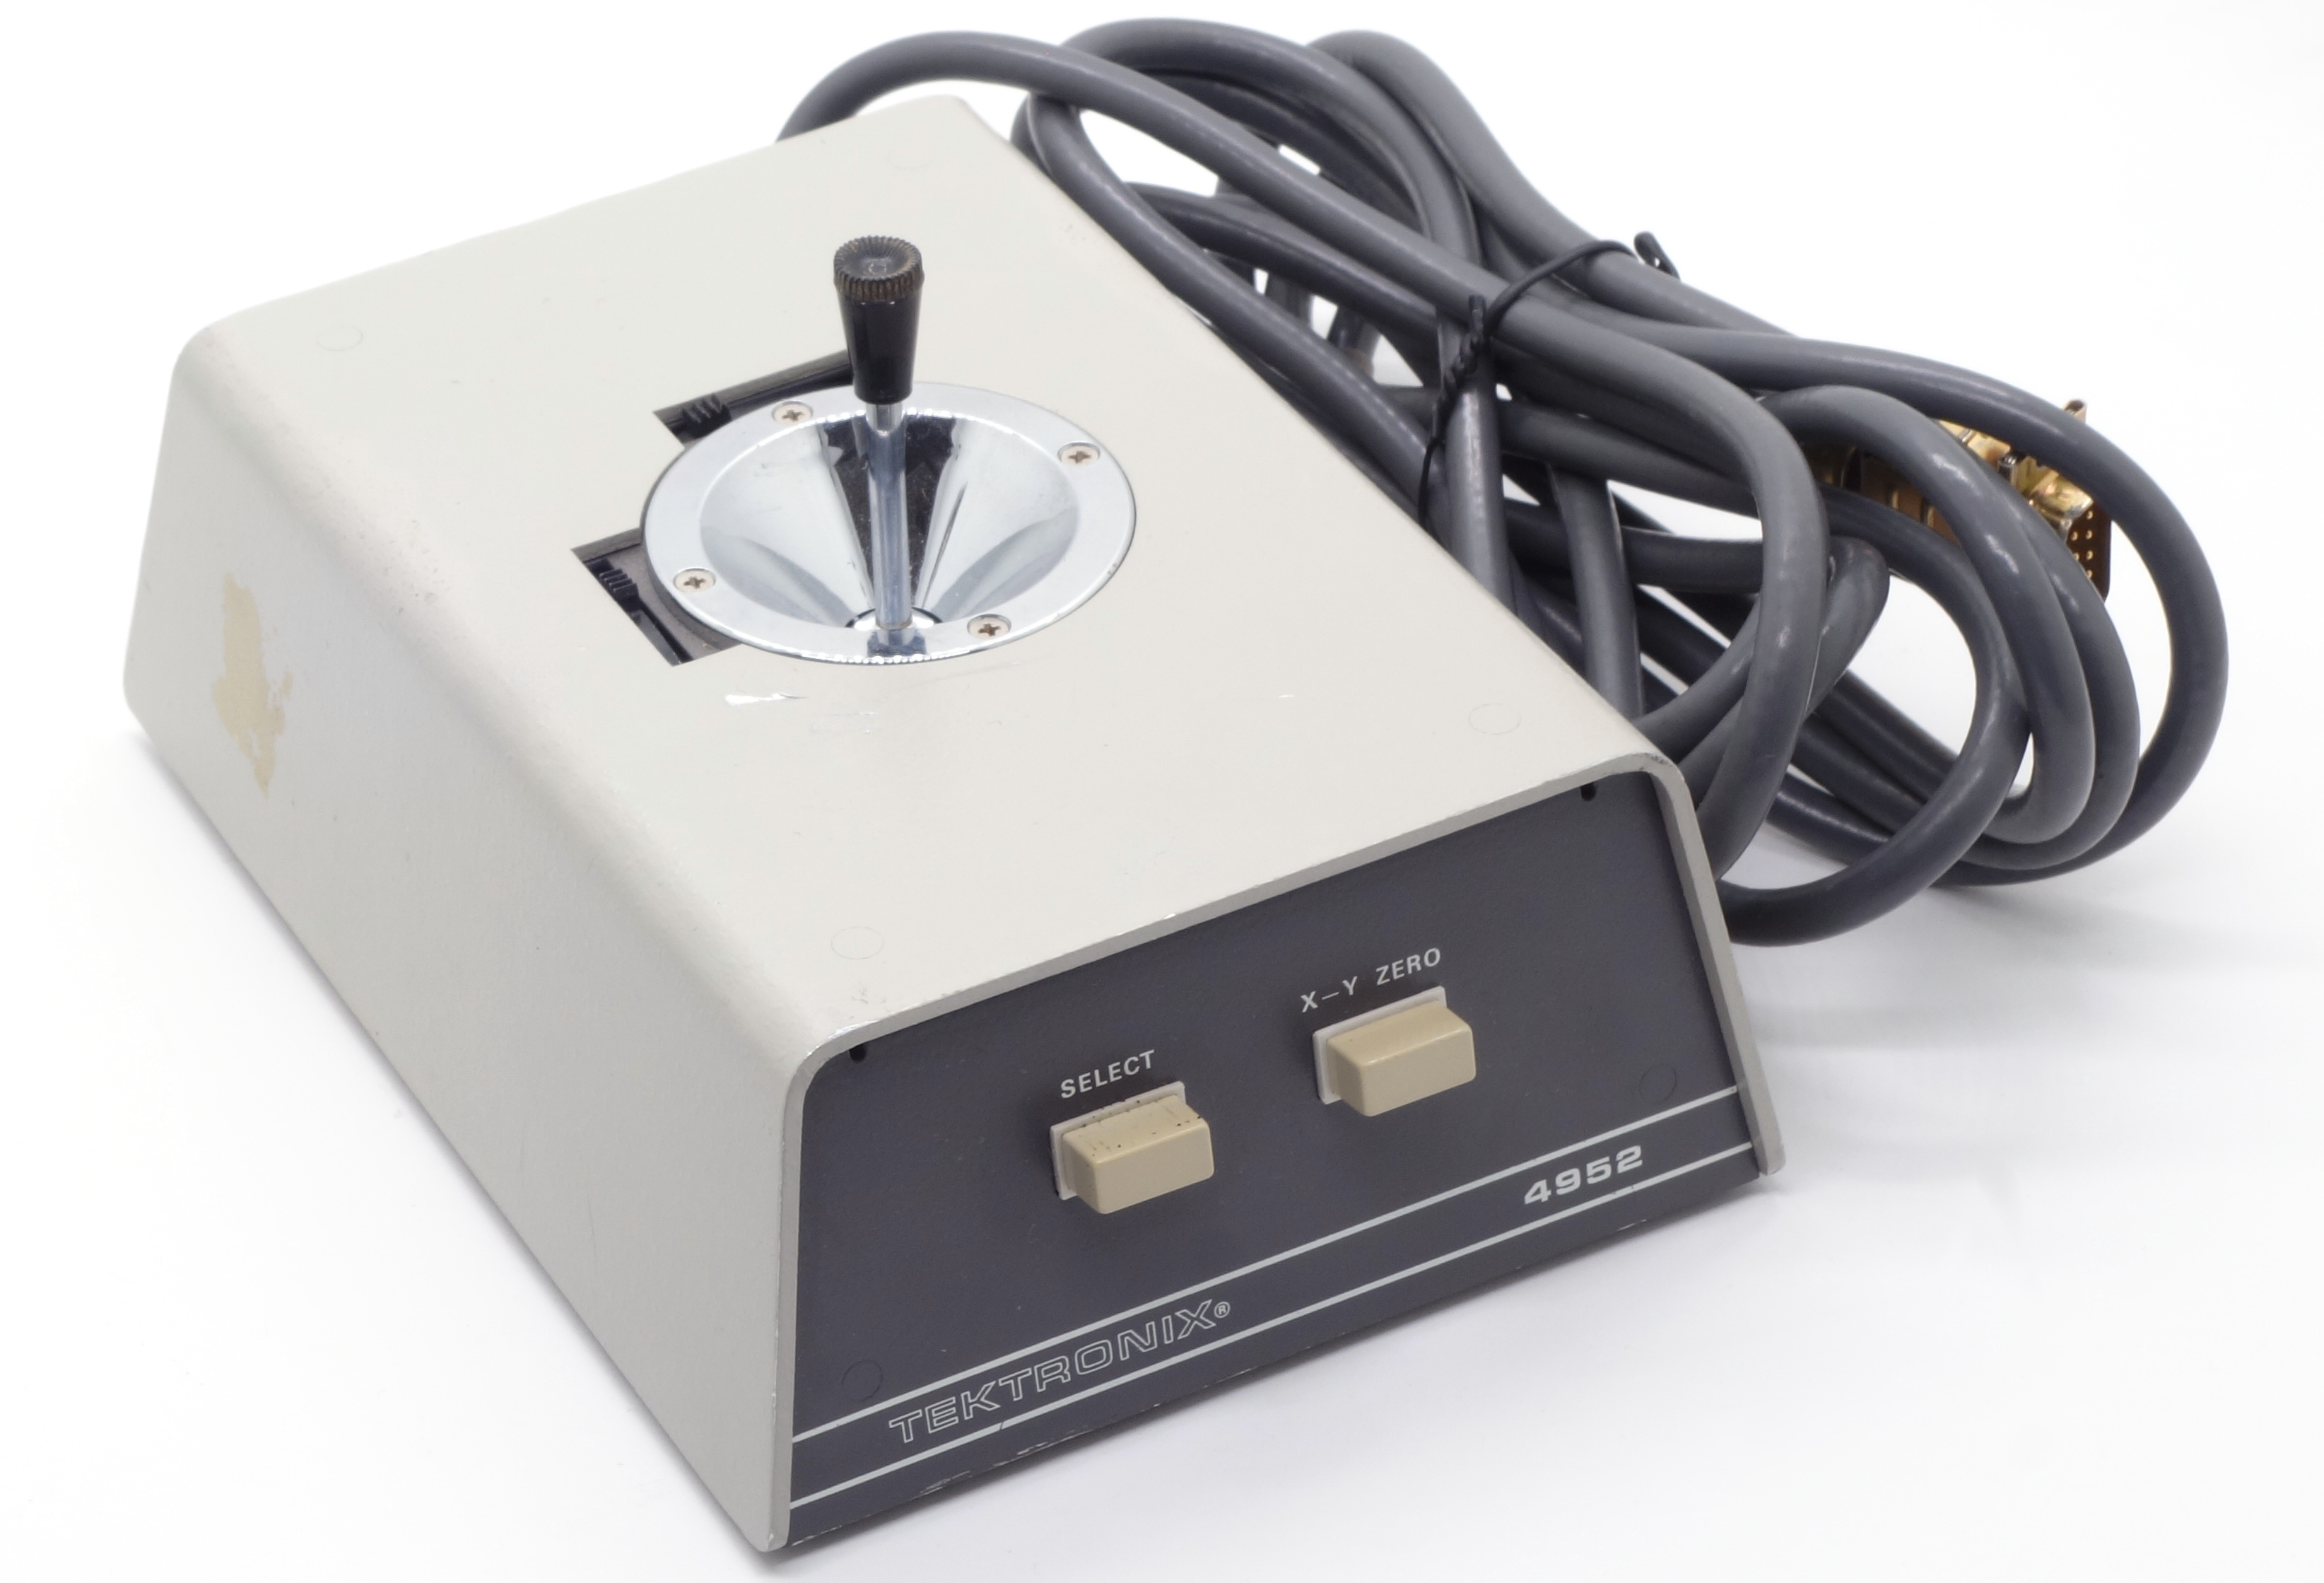
\includegraphics[scale=0.66]{1975_Tektronix_4952_Joystick/pic_30.jpg}
    \caption{Tandy Color Joystick}
    \label{fig:TektronixJoystickPic}
\end{figure}

\begin{figure}[h]
    \centering
    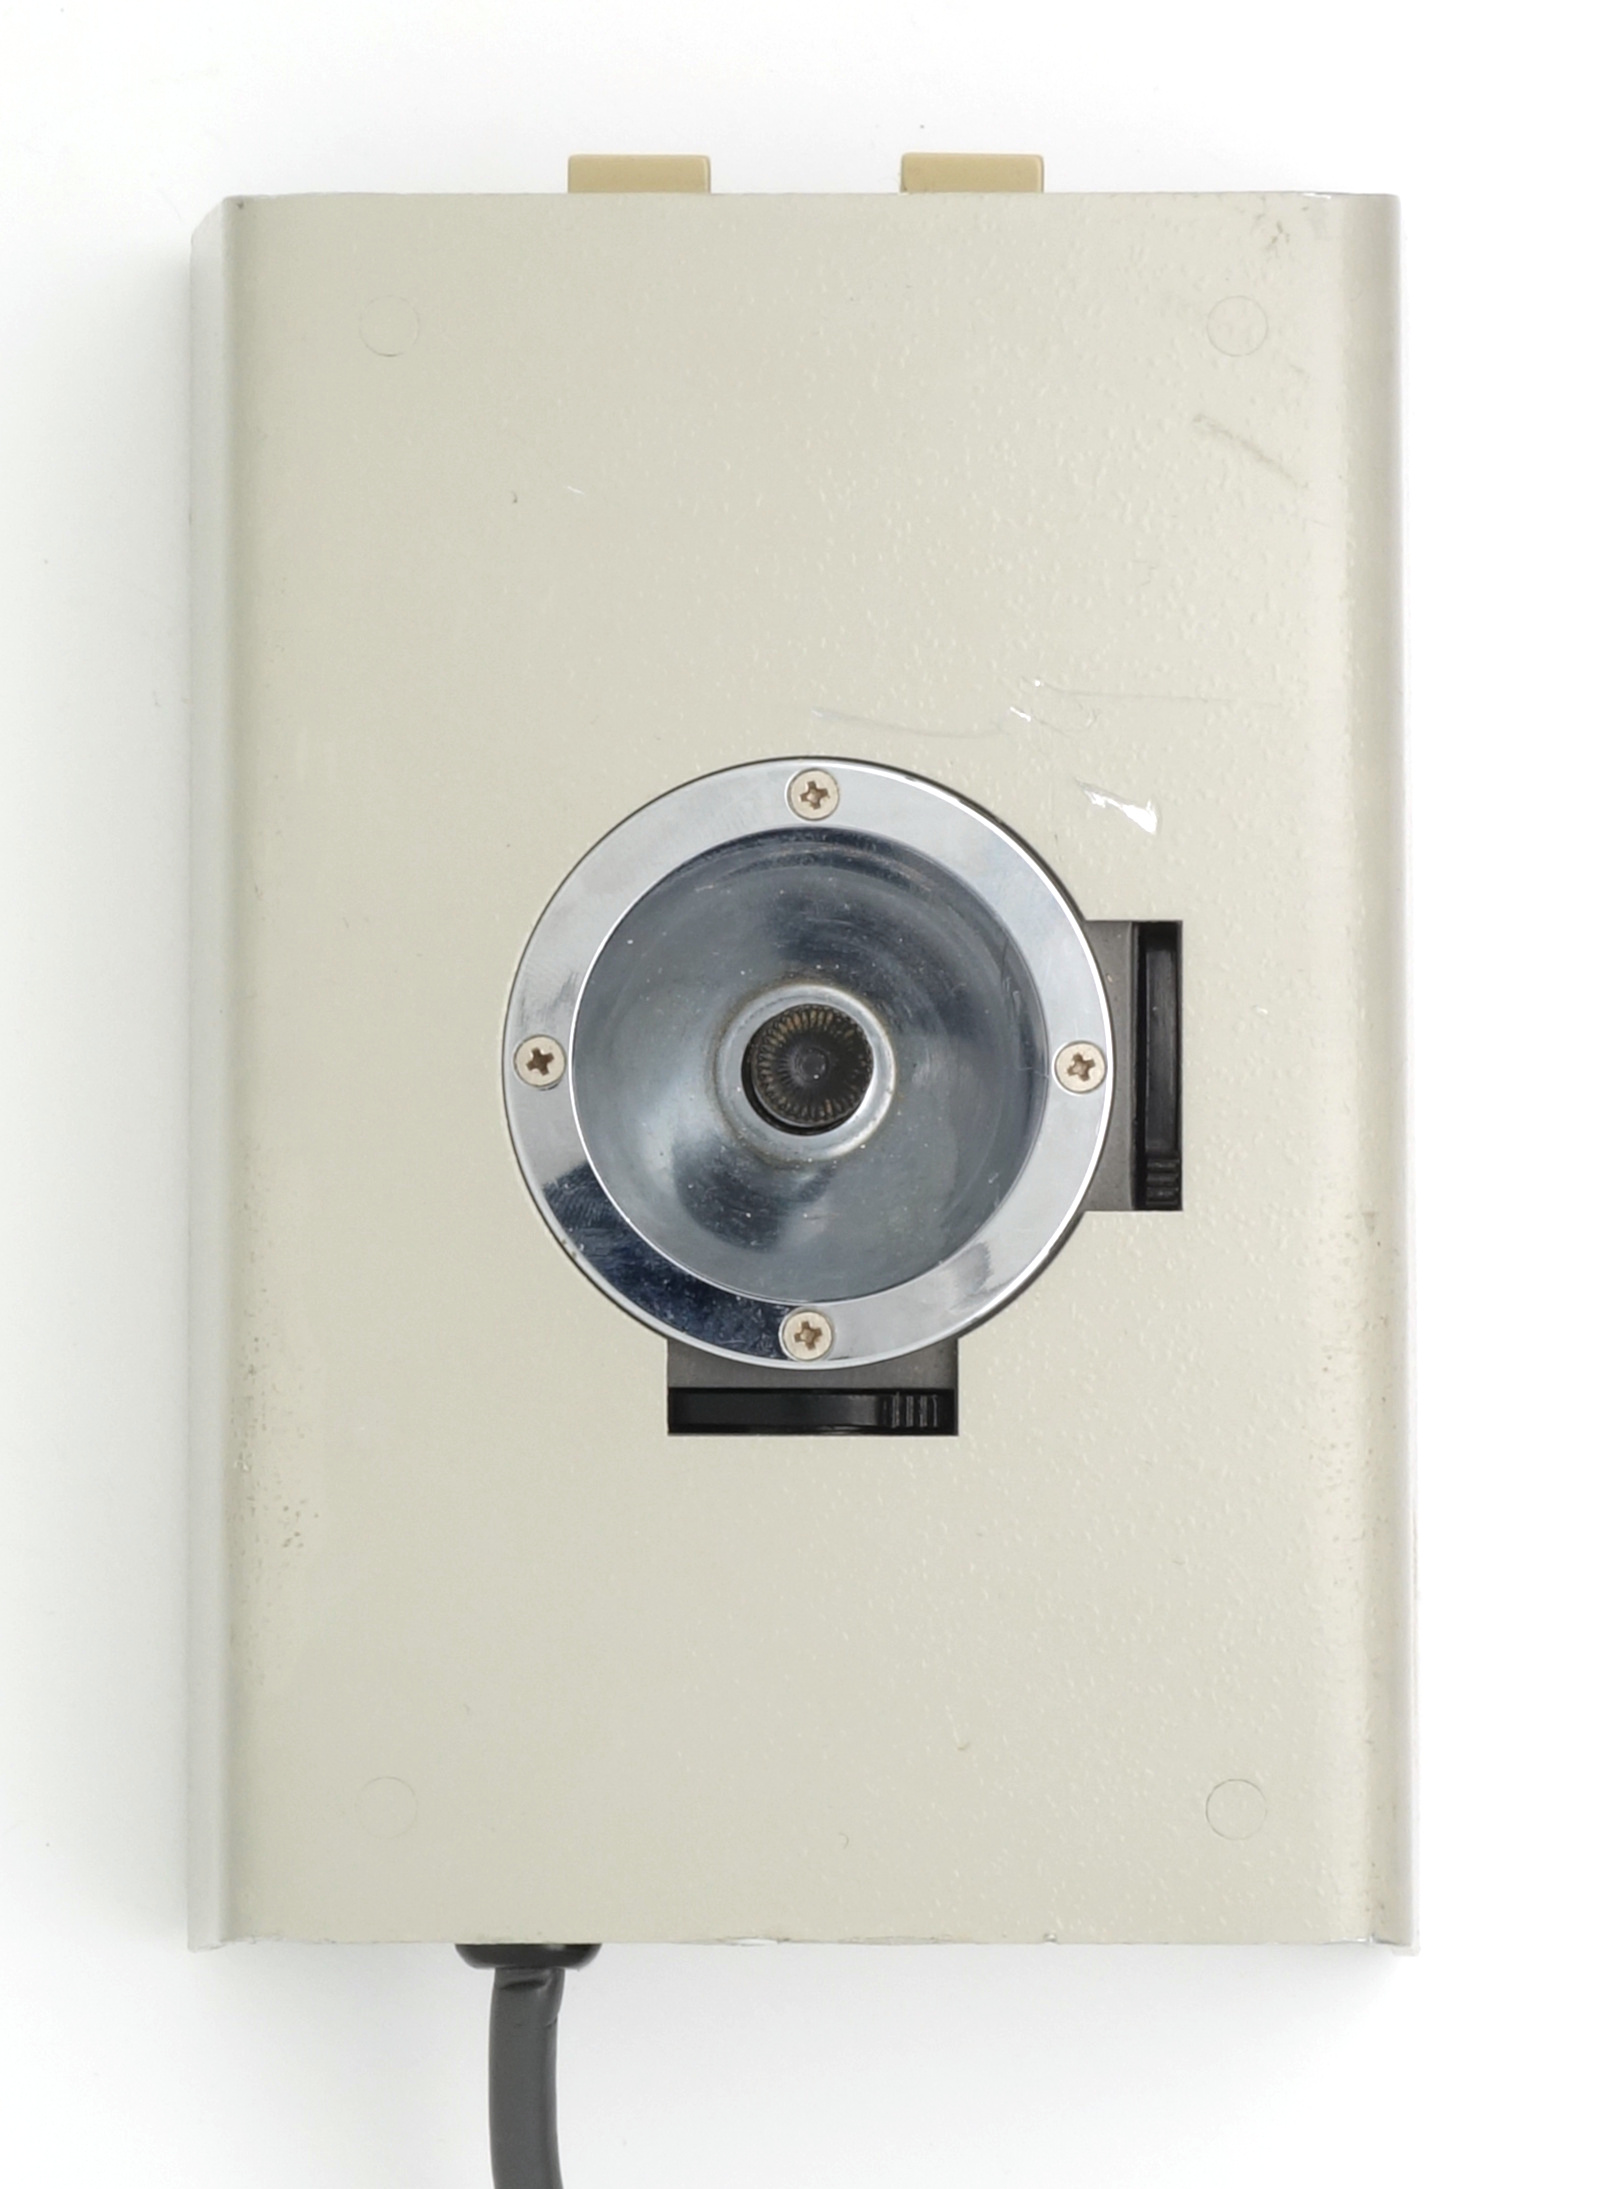
\includegraphics[scale=0.55]{1975_Tektronix_4952_Joystick/top_30.jpg}
    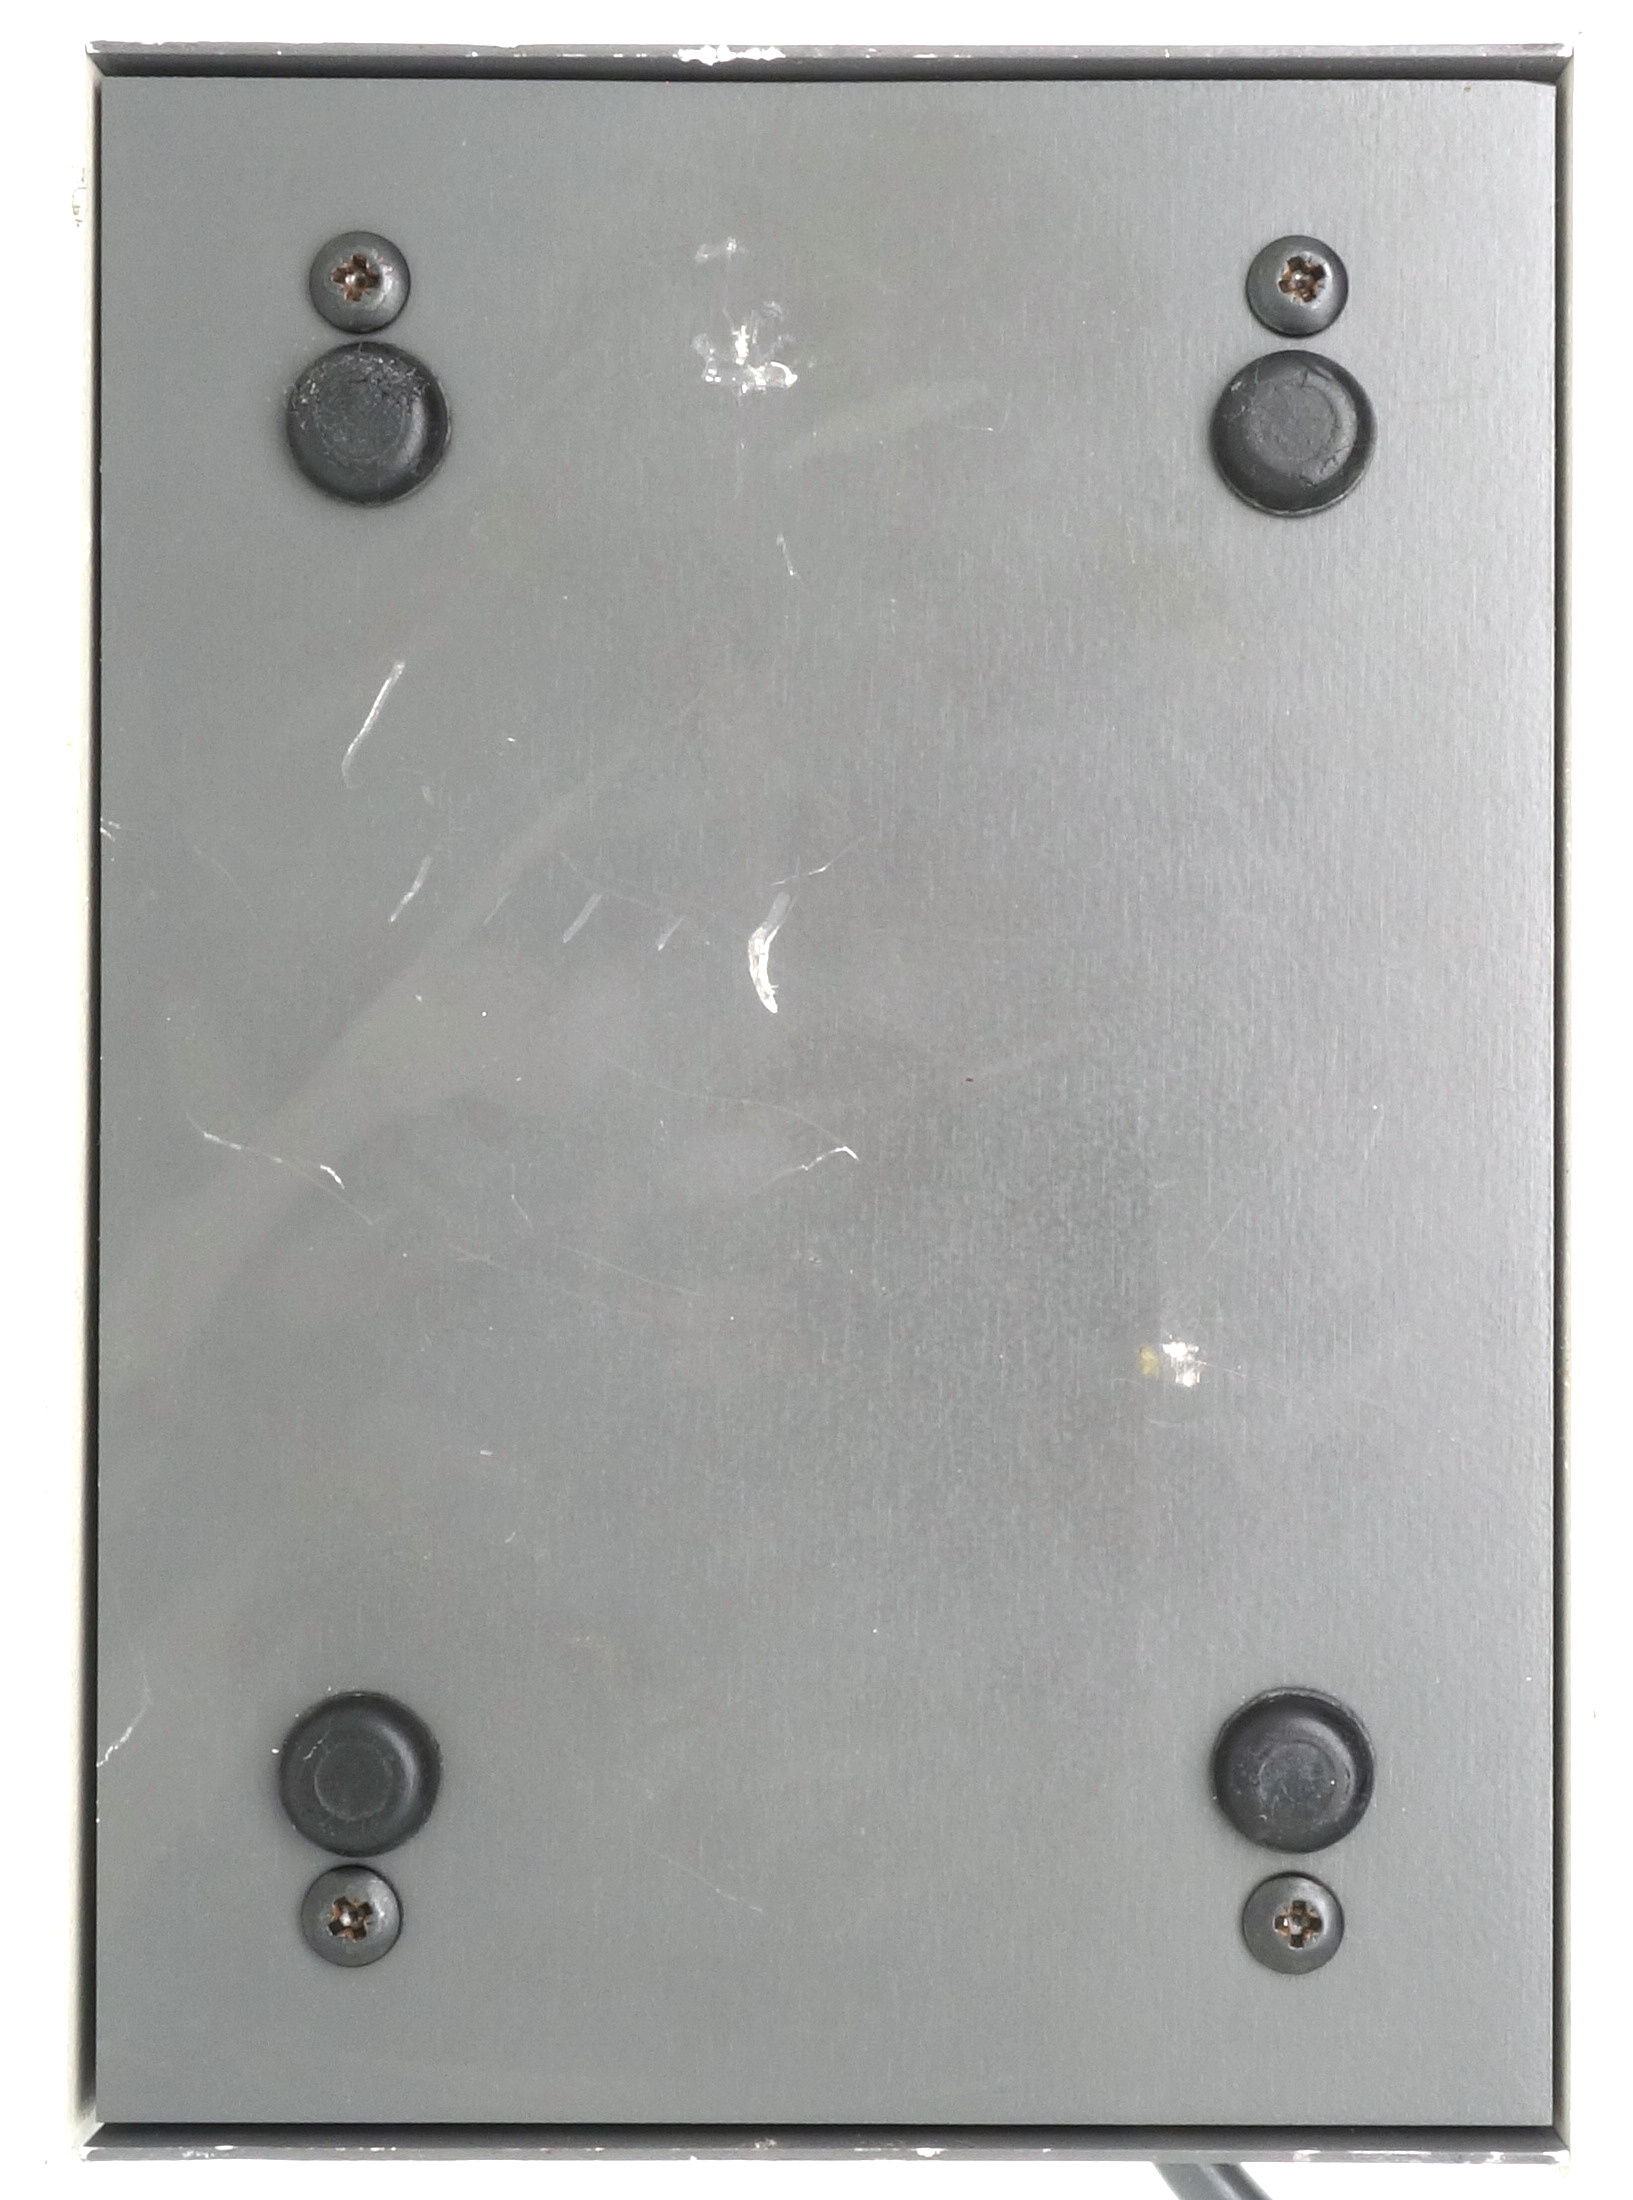
\includegraphics[scale=0.55]{1975_Tektronix_4952_Joystick/bottom_30.jpg}
    \caption{Tandy Color Joystick, top and bottom views}
    \label{fig:TektronixJoystickTopAndBottom}
\end{figure}

The Joystick has a single button (fig. \ref{fig:TektronixJoystickTopAndBottom}) similar in shape to that of the Apple Lisa Joystick released a year earlier, and the body very closely reproduces the shape of another 1983 Joystick -- Sharp MZ-1X10, also manufactured by Alps. The black and red color scheme of the Color Joystick follows the base model of the Tandy Color Computer joystick \cite{hierophant}.

The bottom side shows exactly the same steel ball as the MZ-1X10 has. However, the design of the Color Joystick is much cheaper compared to it: there are no metal balls used as the Joystick feet for easier sliding, and no removable ring which would allow removing the ball for cleaning. The only improvement is a plastic insert that protects the wire from damage in place where it exits the Joystick body.

The Joystick has a small size typical of the 80s (fig. \ref{fig:TektronixJoystickSize}).

\begin{figure}[h]
    \centering
    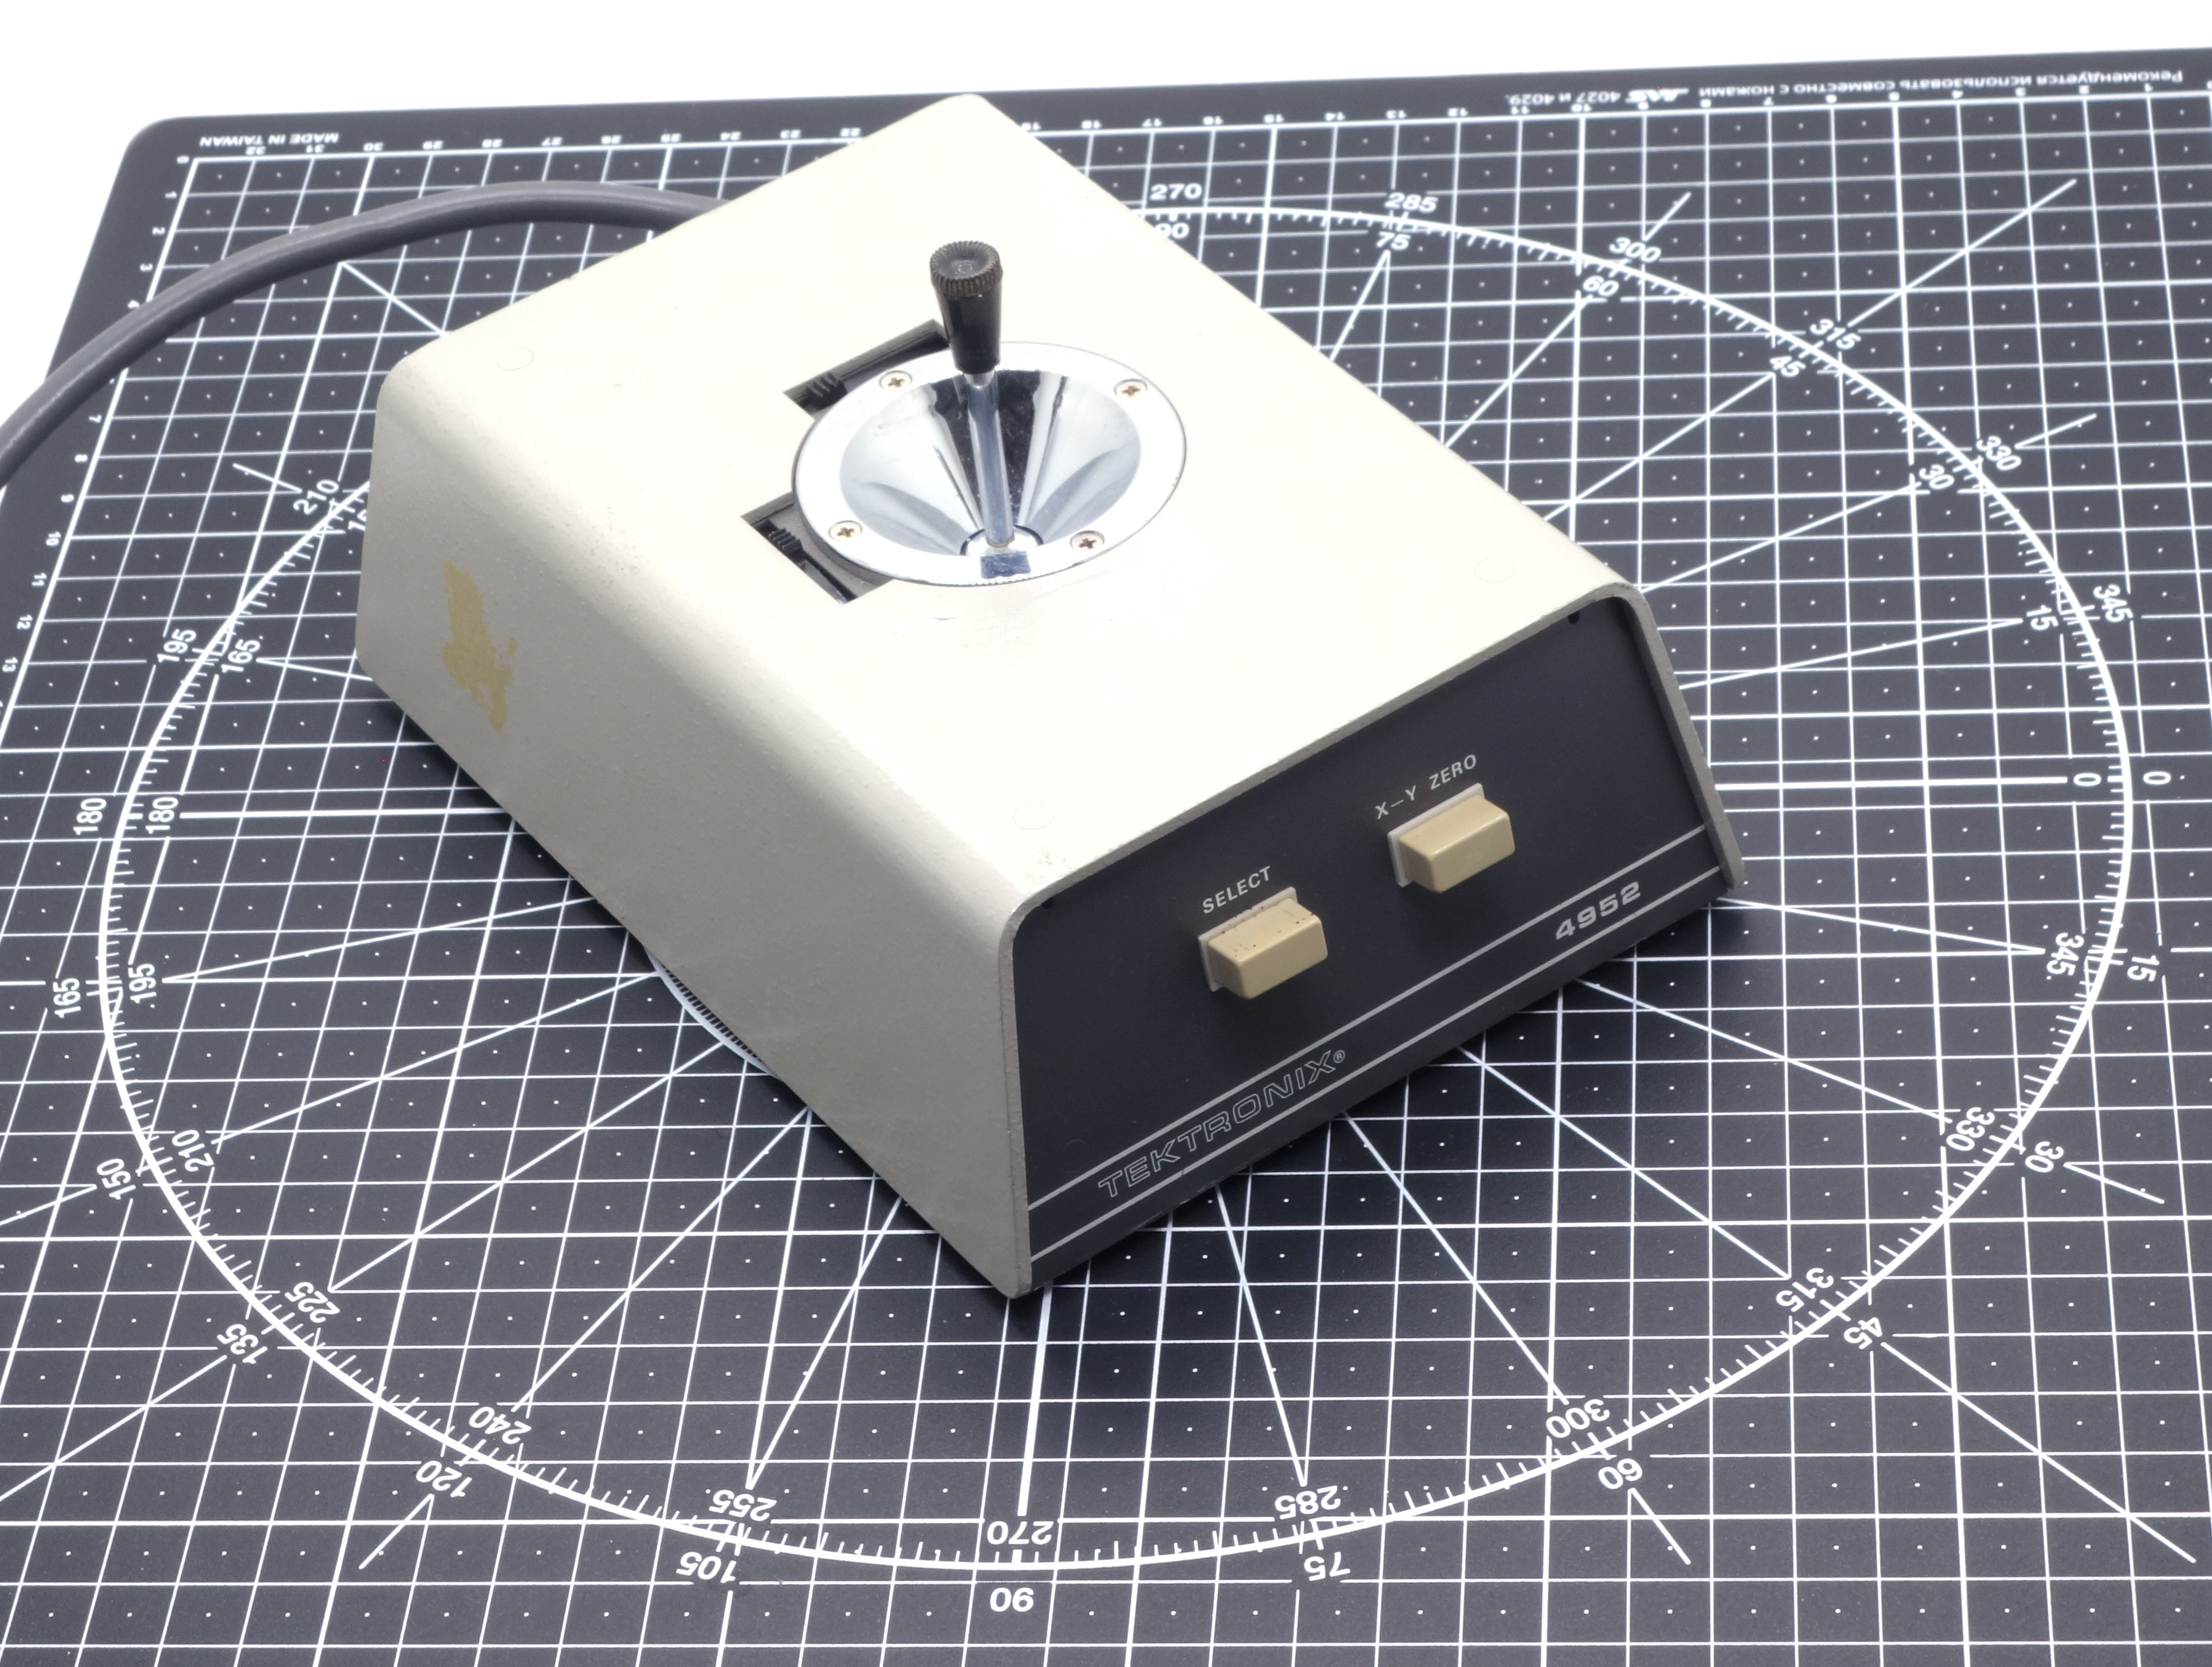
\includegraphics[scale=0.49]{1975_Tektronix_4952_Joystick/size_30.jpg}
    \caption{Tandy Color Joystick on a graduated pad with a grid step of 1~cm}
    \label{fig:TektronixJoystickSize}
\end{figure}

Color Joystick has a fairly simple design; its shape resembles power supply of a player or some other home gadget. Obviously, the beveled back edge should provide a more comfortable palm position, but taking into account the size this does not bring significant improvements to ergonomics (fig. \ref{fig:TektronixJoystickHand}).

As mentioned, the Joystick connects to the analog joystick port. As in the case of a joystick, information about each of the two coordinates is encoded in analog form, by the value of the electrical voltage on the corresponding connector pin. It is stated in the user manual, that Joystick resolution is 64 ``steps'' along each of two coordinate axes \cite{manual}. Such low resolution is caused by the limitations of the Tandy Color Computer analog-to-digital converter: drivers that allow using real analog joysticks to control Joystick cursor were also showing poor positioning accuracy \cite{hierophant}.

\begin{figure}[h]
    \centering
    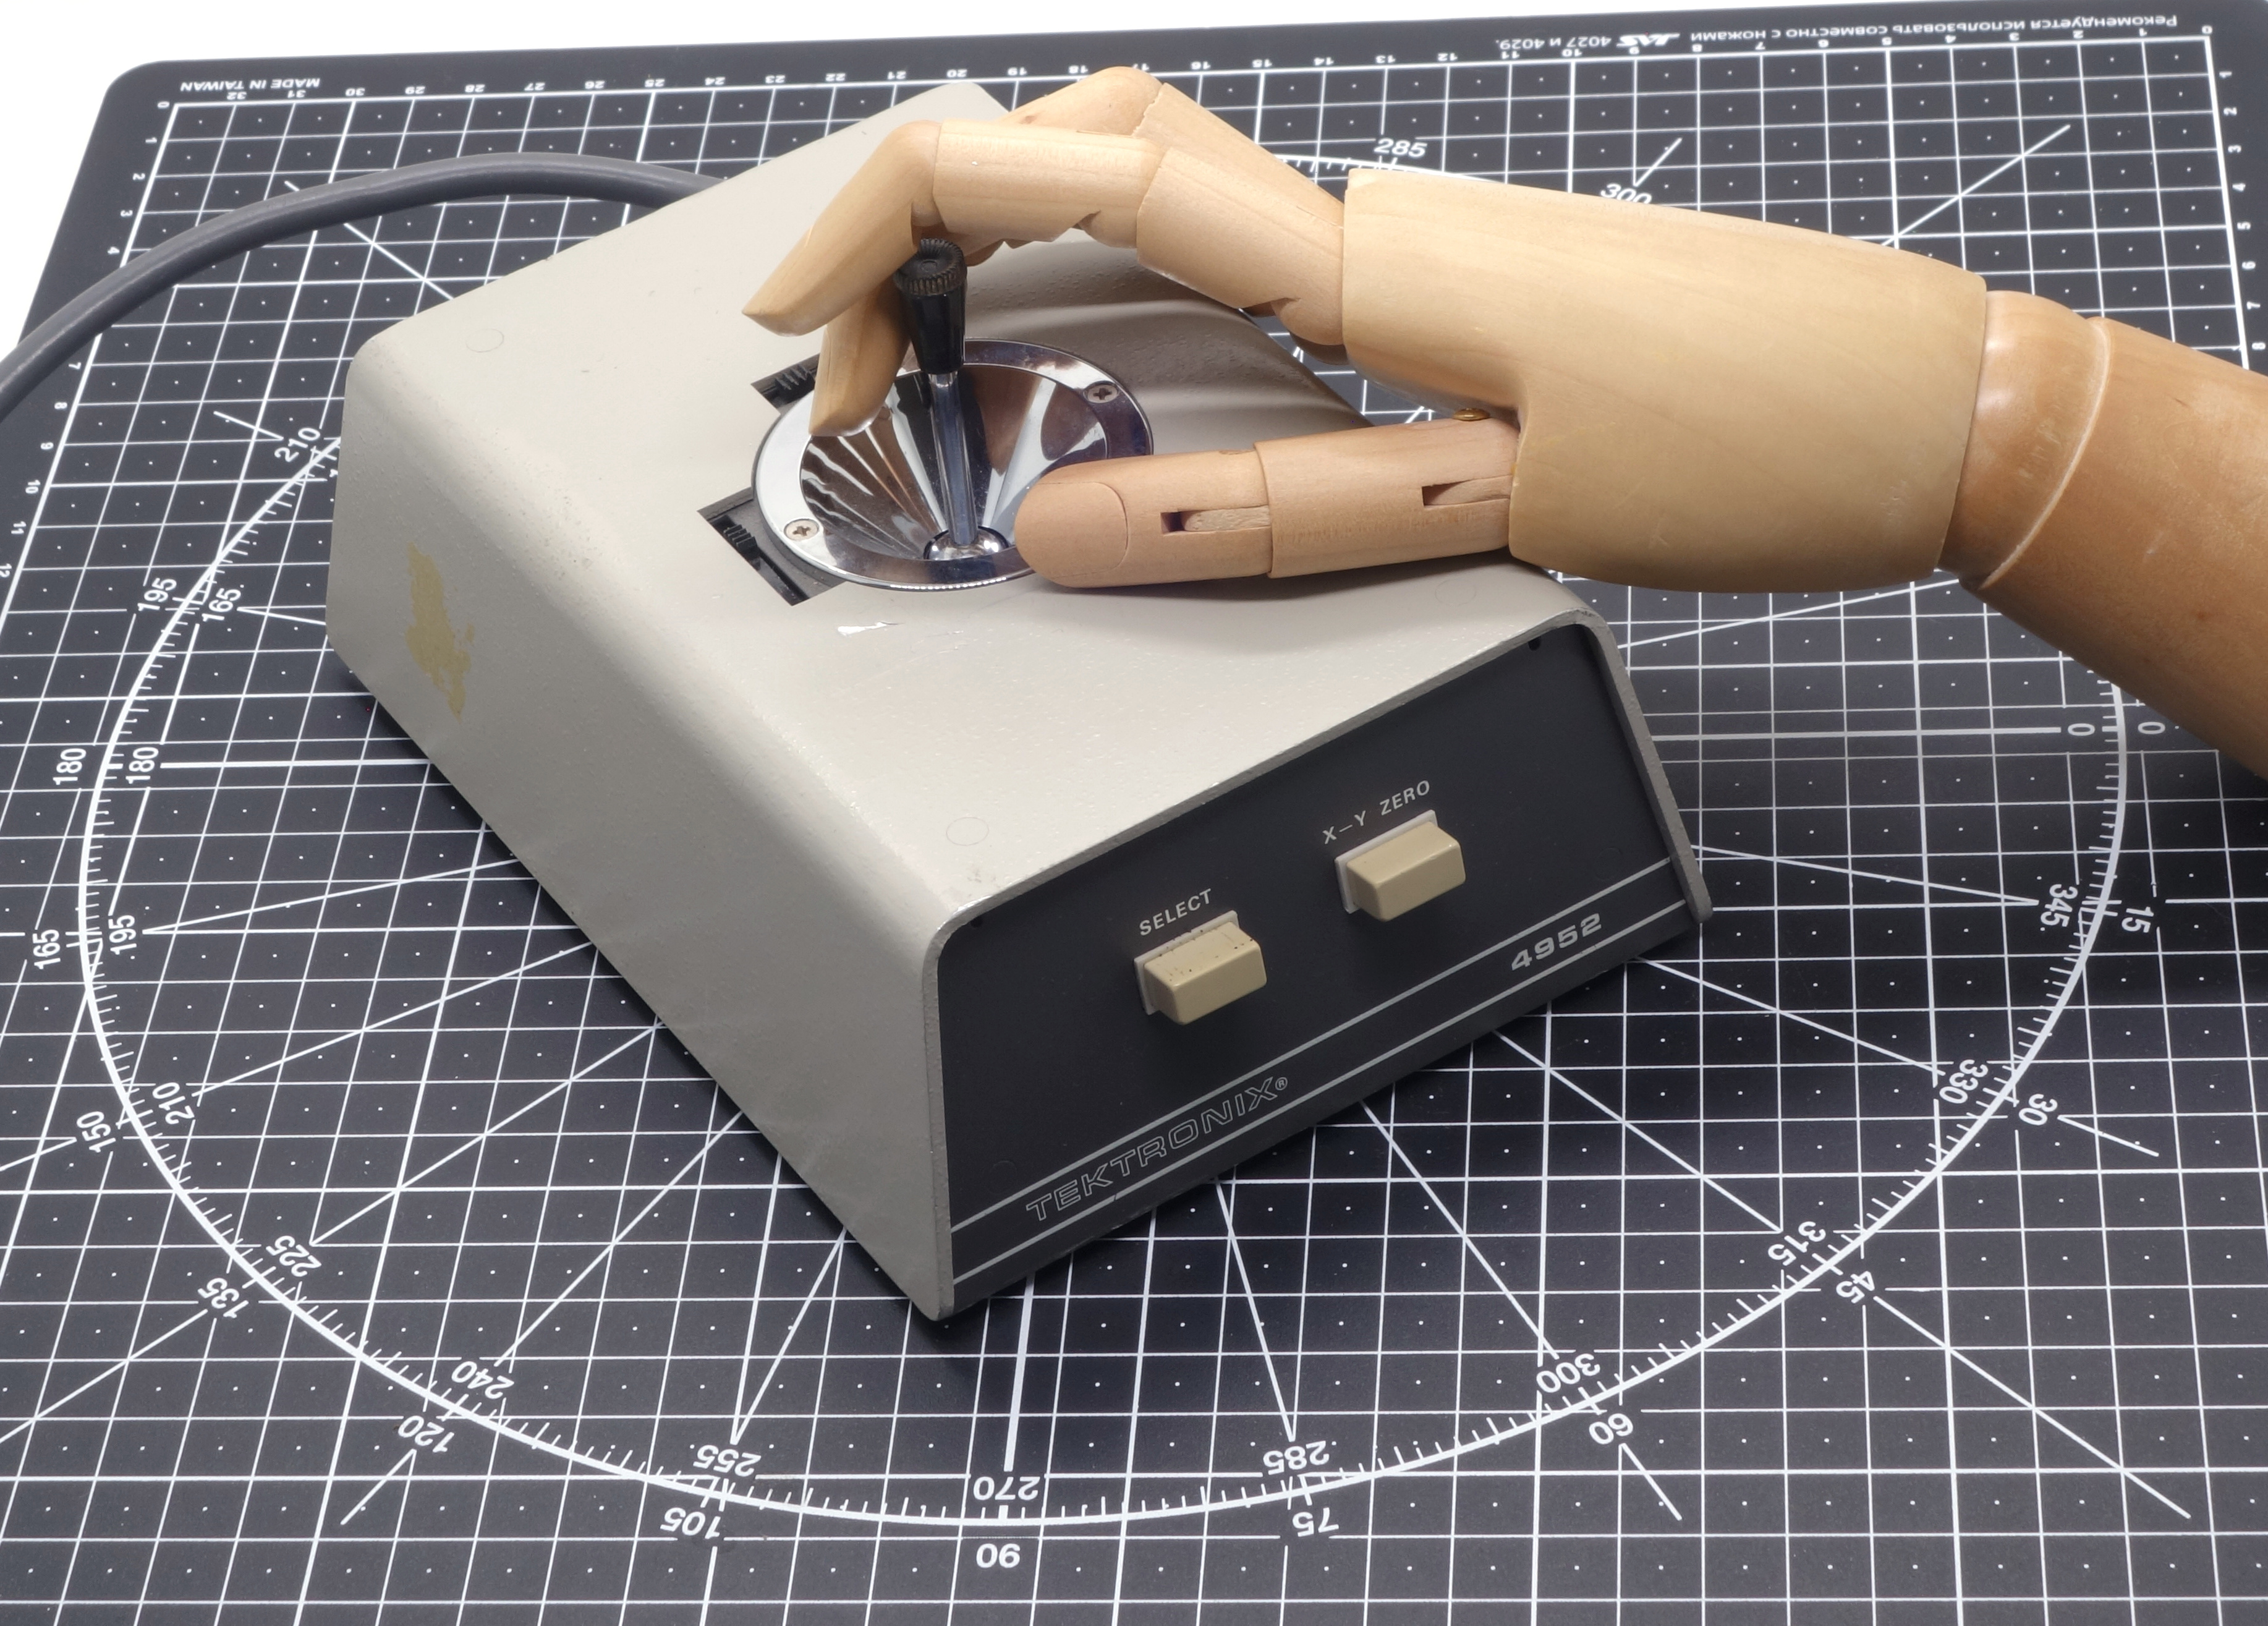
\includegraphics[scale=0.55]{1975_Tektronix_4952_Joystick/hand_05.jpg}
    \caption{Tandy Color Joystick with a human hand model}
    \label{fig:TektronixJoystickHand}
\end{figure}



\begin{figure}[h]
    \centering
    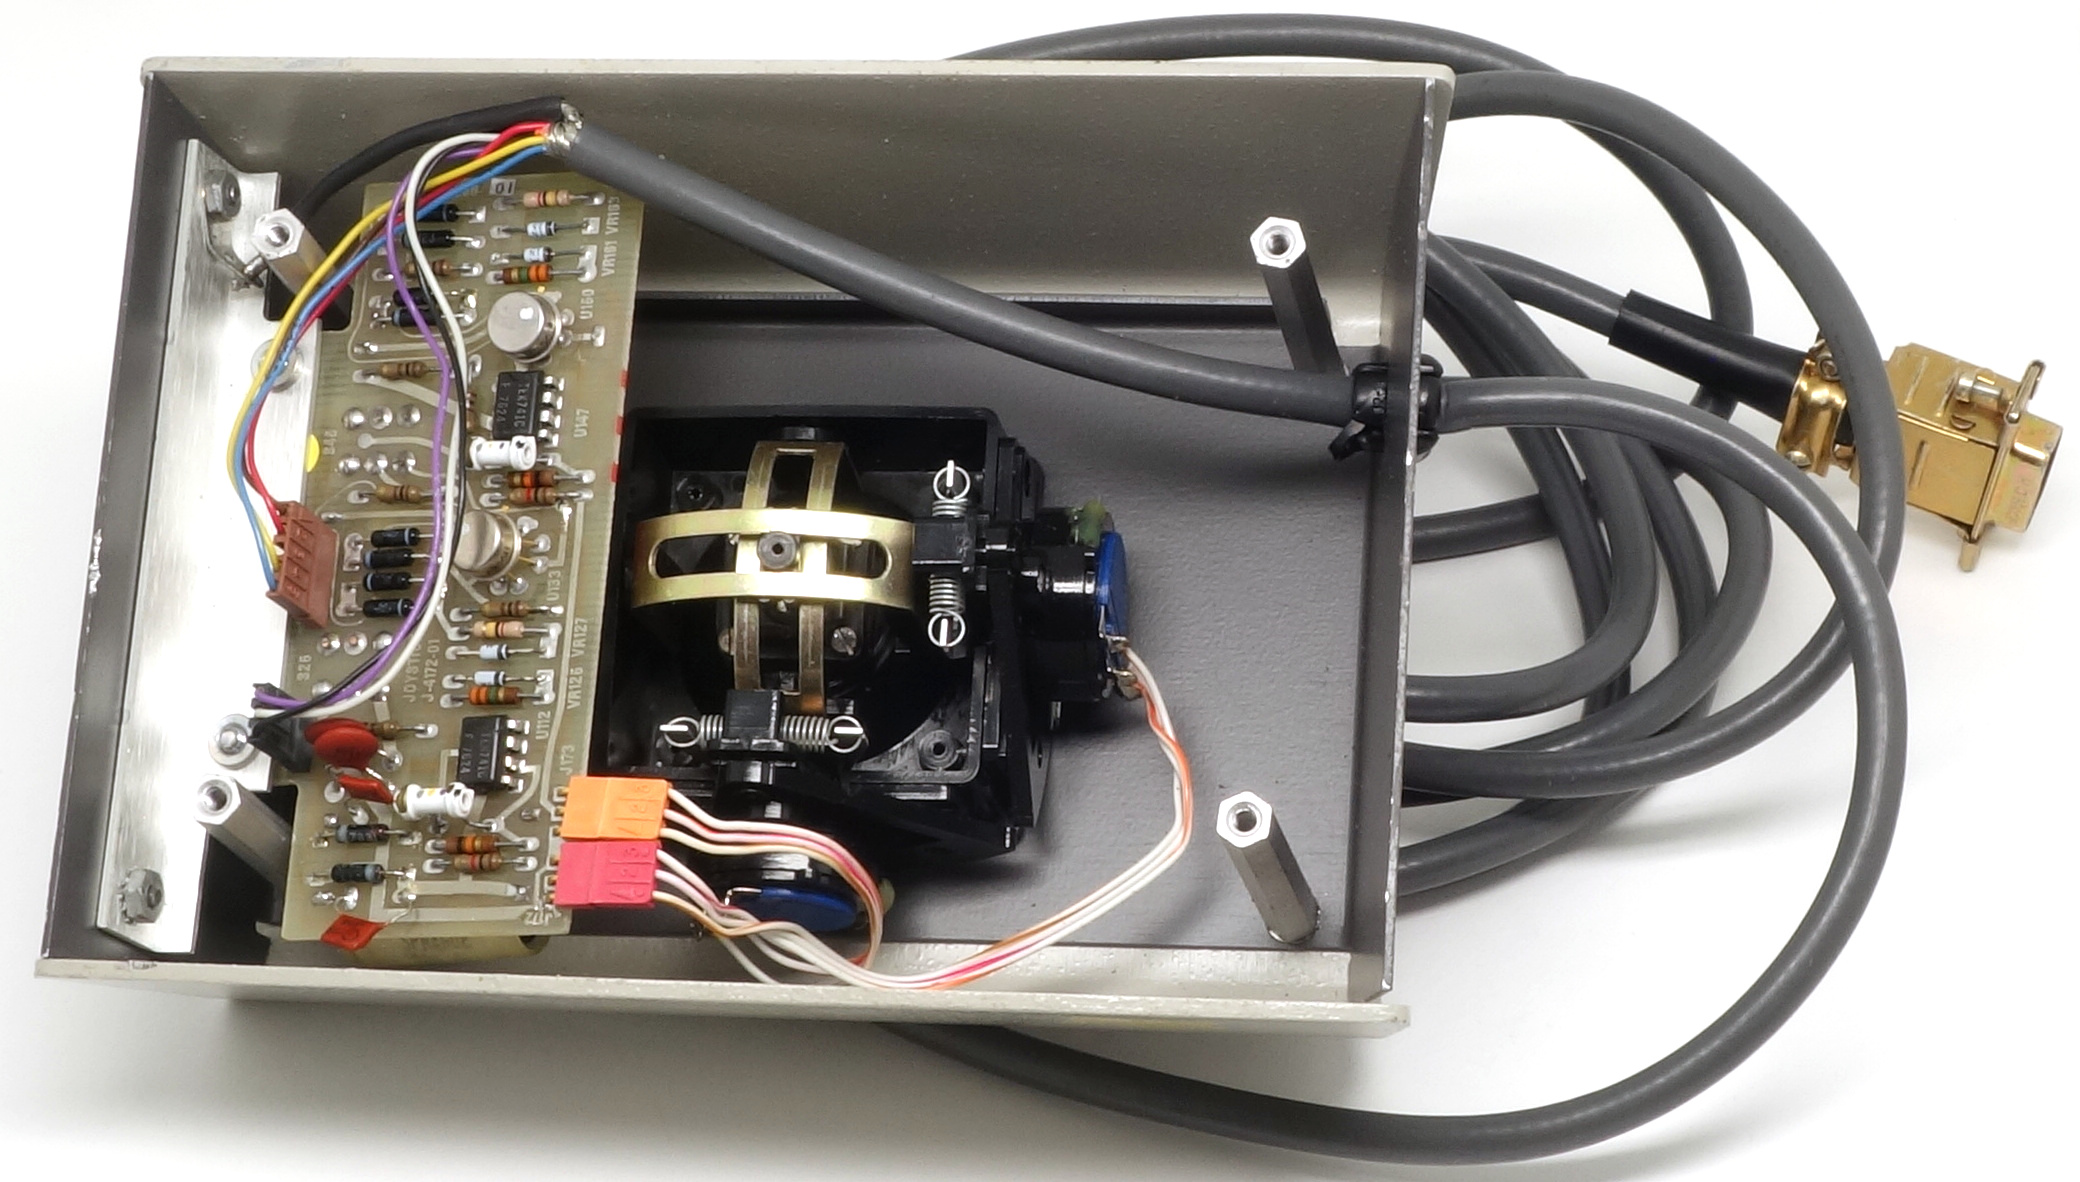
\includegraphics[scale=0.8]{1975_Tektronix_4952_Joystick/inside_30.jpg}
    \caption{Tandy Color Joystick disassembled}
    \label{fig:TektronixJoystickInside}
\end{figure}

Disassembled Joystick is shown in fig. \ref{fig:TektronixJoystickInside}. Tandy Color Joystick does not use contact or optomechanical encoders: instead, the ball transmits motion to a pair of potentiometers, just like an analog joystick stick does. Of course, this solution has significant drawbacks: the Joystick does not allow calibration, and unlike the joystick, the Joystick can't show user that its potentiometers have been moved to the middle position, which should correspond to the location in the center of the Joystick pad, or that they have reached the edge position. However, since Tandy Color Joystick is an absolute coordinate pointing device, user can see location of the cursor on the screen and place the Joystick on more or less appropriate part of the Joystick pad.

\begin{thebibliography}{9}
\bibitem {wiki} Tektronix 4050 -- Wikipedia \url{https://en.wikipedia.org/wiki/Tektronix_4050}
\bibitem {adv} Canadian Information Processing Society (CIPS) Computer Magazine - Vol. 5, Iss. 1-11, 1974. - p. 29
\bibitem {manual} TEKTRONIX 4952 JOYSTICK. Tektronix, Inc., JAN 1975. \url{http://www.bitsavers.org/pdf/tektronix/401x/070-1826-01_4952_Joystick_Jan75.pdf}
\bibitem {price} Stanley J. Tektronix 4952 - Electronixandmore Vintage Electronics and Beyond. -- \url{https://electronixandmore.com/misc/index.php?item=56}
\end{thebibliography}
\end{document}

This joystick went with the 4050-series computer systems and cost \$560 new back in the late seventies. A POINTER statement is used to activate the pointer on the computer, and the joystick would move it around. If any key was pressed, the POINTER statement would end, the X,Y values would be stored, and the key pressed would also be stored.



They are all-in-one designs with the display, keyboard, CPU and tape drive in a single desktop case. They also include a GPIB parallel bus to connect external peripherals. A simple operating system and BASIC interpreter were included in ROM.

T. Several members of the family were introduced during the 1970s, the best known being the 11-inch 4010 and 19-inch 4014, along with the less popular 25-inch 4016. They were widely used in the CAD market in the 1970s and early 1980s, until the introduction of inexpensive graphics workstations in the 1980s.

Other devices in the lineup included the 4951 Joystick. This hardware allowed the user to select any point on a display, and to input its coordinates to a computer, allowing support of a CAD system. 


Canadian Information Processing Society (CIPS) Computer Magazine - Vol. 5, Iss. 1-11, 1974. - p. 29


A new graphics input device, the 4952 Joystick, is being introduced by Tektronix, Inc., to enhance the graphics capabilities of the Tektronix line of computer display terminals, including the 4010, 4012, 4013, 4014 and 4015. The Joystick will generate a a cross-hair cursor which can be positioned to any point on the  terminal's display screen. The graphic address at the cross-hair intersection is then digitized and the X and Y.
The new Tektronix 4952 Joystick, in foreground, is used to enhance the graphics capabilities of the Tektronix line of computer display terminals, such as the 4014 19-inch terminal shown in the background. The Joystick will also operate with the
1 , 4015 , and 4015-1 . The The 4952 Joystick is compatible with 4952 Option 1 is compatible with the 4010 , 4010-1 , 4012 and 4013. Both Joysticks come with an 11-1/2 foot cable. The Canadian duty free selling price is \$550.00

